\documentclass[12pt,a4paper]{article}
\usepackage[a4paper, margin=0.8in, headheight=14pt]{geometry}
\usepackage{fontspec}
\usepackage{unicode-math}
\setmainfont{TeX Gyre Pagella}
\setmonofont[Scale=0.88]{TeX Gyre Cursor}
\setmathfont{Latin Modern Math}
\usepackage{xcolor}
\usepackage{colortbl}
\usepackage{titlesec}
\usepackage{enumitem}
\usepackage{tabularx}
\usepackage{booktabs}
\usepackage{array}
\usepackage{amsmath}
\allowdisplaybreaks
\usepackage{tikz}
\usetikzlibrary{shapes.geometric, arrows.meta, positioning, calc, fit, decorations.pathreplacing, decorations.pathmorphing, patterns, backgrounds}
% circuitikz not required for this subject
\usepackage{tcolorbox}
\tcbuselibrary{skins, breakable}
\usepackage{etoolbox}
\usepackage{hyperref}
\usepackage{fancyhdr}
\usepackage{graphicx}
\usepackage{microtype}
\hyphenpenalty=10000
\exhyphenpenalty=10000
\sloppy
\usepackage{caption}
\usepackage{setspace}
\usepackage{multirow}
\usepackage{tocloft}
\newcommand{\Q}[1]{\textbf{#1}\par\noindent\ignorespaces}
\definecolor{myred}{RGB}{196,30,58}
\definecolor{mydark}{RGB}{30,30,50}
\definecolor{mygreen}{RGB}{14,120,80}
\definecolor{myteal}{RGB}{0,130,140}
\definecolor{myamber}{RGB}{180,100,0}
\definecolor{mypurple}{RGB}{100,30,160}
\definecolor{mygray}{RGB}{246,247,249}
\definecolor{mgframe}{RGB}{180,185,200}
\definecolor{watermark}{RGB}{145,150,170}
\definecolor{hdrred}{RGB}{250,232,235}
\definecolor{hdrgreen}{RGB}{220,244,233}
\definecolor{hdrteal}{RGB}{220,242,244}
\definecolor{hdramber}{RGB}{253,242,215}
\definecolor{hdrpurple}{RGB}{238,228,255}
\definecolor{hdrgray}{RGB}{238,240,245}
\AfterEndEnvironment{tcolorbox}{\color{mydark}}

\titleformat{\section}{\large\bfseries\color{myred}}{\thesection.}{0.5em}{}[\vspace{1pt}{\color{myred}\rule{\linewidth}{0.8pt}}]
\titleformat{\subsection}{\normalsize\bfseries\color{myteal}}{\thesubsection}{0.5em}{}
\titlespacing*{\section}{0pt}{18pt}{7pt}
\titlespacing*{\subsection}{0pt}{11pt}{4pt}
\setlength{\parindent}{0pt}
\setlength{\parskip}{4pt}
\renewcommand{\cfttoctitlefont}{\large\bfseries\color{myred}}
\renewcommand{\cftaftertoctitle}{\par\noindent{\color{myred}\rule{\linewidth}{0.8pt}}}
\setlength{\cftbeforetoctitleskip}{0pt}
\setlength{\cftaftertoctitleskip}{6pt}
\renewcommand{\cftsecfont}{\normalsize\bfseries\color{mydark}}
\renewcommand{\cftsecpagefont}{\normalsize\bfseries\color{mydark}}
\renewcommand{\cftsecleader}{\cftdotfill{\cftdotsep}}
\setlength{\cftbeforesecskip}{5pt}
\renewcommand{\cftsubsecfont}{\small\color{mydark}}
\renewcommand{\cftsubsecpagefont}{\small\color{mydark}}
\setlength{\cftbeforesubsecskip}{2pt}
\setlength{\cftsubsecindent}{1.4em}
\renewcommand{\cftpartfont}{\normalsize\bfseries\color{myteal}}
\renewcommand{\cftpartpagefont}{\normalsize\bfseries\color{myteal}}
\setlength{\cftbeforepartskip}{10pt}
\renewcommand{\arraystretch}{1.45}
\setlength{\tabcolsep}{6pt}
\arrayrulecolor{mydark}
\newcolumntype{B}[1]{>{\small\bfseries\raggedright\arraybackslash}m{#1}}
\newcolumntype{C}[1]{>{\centering\arraybackslash}m{#1}}
\newcolumntype{Y}{>{\small\raggedright\arraybackslash}X}
\renewcommand{\tabularxcolumn}[1]{m{#1}}
\newcommand{\currmodule}{Module 1}
\pagestyle{fancy}
\fancyhf{}
\fancyhead[L]{\small\color{myred}\textbf{BS-M401}\;\color{mydark}--- Numerical Methods}
\fancyhead[R]{\small\color{myteal}\textbf{\currmodule\ Notes}}
\fancyfoot[C]{\small\color{mydark}\thepage}
\fancyfoot[R]{\small\color{watermark}\textit{\copyright\ Biraj}}
\renewcommand{\headrulewidth}{0.5pt}
\renewcommand{\footrulewidth}{0.3pt}

\hypersetup{colorlinks=true, linkcolor=myteal, urlcolor=myteal,
  pdfauthor={Biraj Sarkar},
  pdftitle={BS-M401 --- Combined Notes}}

\tcbset{
  tikzbox/.style={
    colback=mygray, colframe=mgframe, boxrule=0.6pt, arc=4pt,
    left=8pt, right=8pt, top=6pt, bottom=6pt,
    colbacktitle=mgframe, coltitle=mydark, fonttitle=\small\bfseries
  },
  defbox/.style={
    colback=hdrgreen, colframe=mygreen, boxrule=0.8pt, arc=4pt,
    left=9pt, right=9pt, top=6pt, bottom=6pt,
    colbacktitle=mygreen, coltitle=white, fonttitle=\small\bfseries
  },
  formulabox/.style={
    colback=hdrteal, colframe=myteal, boxrule=0.8pt, arc=4pt,
    left=9pt, right=9pt, top=7pt, bottom=7pt,
    colbacktitle=myteal, coltitle=white, fonttitle=\small\bfseries
  },
  examplebox/.style={
    colback=hdramber, colframe=myamber, boxrule=0.8pt, arc=4pt,
    left=9pt, right=9pt, top=6pt, bottom=6pt,
    colbacktitle=myamber, coltitle=white, fonttitle=\small\bfseries
  },
  masonbox/.style={
    colback=hdrpurple, colframe=mypurple, boxrule=0.8pt, arc=4pt,
    left=9pt, right=9pt, top=6pt, bottom=6pt,
    colbacktitle=mypurple, coltitle=white, fonttitle=\small\bfseries
  },
  exambox/.style={
    colback=hdrpurple, colframe=mypurple, boxrule=1pt, arc=5pt,
    left=10pt, right=10pt, top=8pt, bottom=8pt,
    colbacktitle=mypurple, coltitle=white, fonttitle=\bfseries,
    breakable, title after break={\textbf{Frequently Asked / Viva Questions (contd.)}}
  }
}
\tcbset{breakable}
\tcbset{coltext=mydark}
\tcbset{after={\color{mydark}}}

\tikzset{
  block/.style={rectangle, draw=myteal, fill=hdrteal,
    text width=2.4cm, align=center, minimum height=0.95cm,
    font=\small, rounded corners=3pt, line width=0.7pt},
  redblock/.style={rectangle, draw=myred, fill=hdrred,
    text width=2.4cm, align=center, minimum height=0.95cm,
    font=\small, rounded corners=3pt, line width=0.7pt},
  amberblock/.style={rectangle, draw=myamber, fill=hdramber,
    text width=2.4cm, align=center, minimum height=0.95cm,
    font=\small, rounded corners=3pt, line width=0.7pt},
  sumjunc/.style={circle, draw=myamber, fill=hdramber,
    minimum size=0.62cm, font=\small, line width=0.8pt},
  arrow/.style={-Stealth, thick, color=mydark},
  redarrow/.style={-Stealth, thick, color=myred},
  line/.style={thick, color=mydark}
}

\newcommand{\modulestart}[2]{%
  \clearpage
  \renewcommand{\currmodule}{Module #1}%
  \renewcommand{\theHsection}{mod#1.\arabic{section}}%
  \renewcommand{\theHsubsection}{\theHsection.\arabic{subsection}}%
  \renewcommand{\theHsubsubsection}{\theHsubsection.\arabic{subsubsection}}%
  \phantomsection
  \addcontentsline{toc}{part}{Module #1: #2}%
  \setcounter{section}{0}%
  \begin{center}
    \vspace*{1.0cm}
    {\Huge\bfseries\color{myred} Module #1}\\[10pt]
    {\Large\bfseries\color{mydark} #2}\\[10pt]
    {\color{myred}\rule{0.55\linewidth}{1.2pt}}
  \end{center}
  \vspace{14pt}
}
\begin{document}

\thispagestyle{empty}

% ─── Page Border (TikZ Overlay) ────────────────────────────────────────────────
\begin{tikzpicture}[remember picture, overlay]
  % Outer border (fine line in mgframe)
  \draw[color=mgframe, line width=1.5pt] 
    ($(current page.north west) + (0.6in, -0.6in)$) rectangle 
    ($(current page.south east) + (-0.6in, 0.6in)$);
  % Inner border (finer accent line in myred)
  \draw[color=myred, line width=0.8pt] 
    ($(current page.north west) + (0.65in, -0.65in)$) rectangle 
    ($(current page.south east) + (-0.65in, 0.65in)$);
\end{tikzpicture}

\vspace*{1.0cm}
\begin{center}
  {\Huge\bfseries\color{myred} BS-M401}\\[10pt]
  {\LARGE\bfseries\color{mydark} Numerical Methods}\\[20pt]
  {\color{myred}\rule{0.7\linewidth}{1.5pt}}\\[18pt]
  {\Large\color{myteal}\textbf{Combined Module Notes}}\\[8pt]
  {\large\color{mydark} Modules 1 -- 3}\\[40pt]
  {\normalsize\color{mydark} Semester IV \quad$\bullet$\quad ECE \quad$\bullet$\quad 2 Credits}\\[12pt]
  {\normalsize\color{mydark} CGEC \;$|$\; B.Tech ECE (2023--27)}
\end{center}
\vspace{1.0cm}
\begin{center}
  \begin{tcolorbox}[colback=mygray, colframe=mgframe, boxrule=0.5pt, arc=3pt, width=0.85\linewidth]
    \centering\small\color{mydark}
    \textbf{Disclaimer / Study Guide Notice:}\\
    These are condensed \textbf{Short Notes} focusing on core theory, key formulas, block/circuit diagrams, and standard viva Q\&As for university exam revision. Exhaustive numerical practice problems and derivation edge cases are not covered. This serves as a quick-revision reference guide for students.
  \end{tcolorbox}
\end{center}
\vfill
\vspace{0.6cm}
\begin{center}
  {\large\bfseries\color{mypurple} Biraj Sarkar}\\[16pt]
  {\footnotesize\color{watermark}\textbf{IN ASSOCIATION WITH}}\\[8pt]
  {\small\bfseries\color{mydark} MAKAUT Wingman \quad$\bullet$\quad MAKAUT Future Minds}\\[12pt]
  {\large\bfseries\color{myteal} Cooch Behar Government Engineering College}
\end{center}
\vfill
\begin{center}{\small\color{watermark}\textit{Exam-Ready Notes}}\end{center}
\clearpage

\hypersetup{linkcolor=mydark}
\tableofcontents
\hypersetup{linkcolor=myteal}
\clearpage

% -- Module 1 -----------------------------------------------------------------
\modulestart{1}{Numerical Errors, Interpolation and Integration}

\section{Numerical Errors, Interpolation and Integration}
\subsection{Approximation and types of error}
\begin{tcolorbox}[defbox, title={Numerical approximation}]
A numerical method replaces an exact mathematical operation by a finite computation. If $x$ is the true value and $\hat{x}$ its approximation, use the signed-error convention $e=x-\hat{x}$. The absolute error is $|e|$.
\end{tcolorbox}

\begin{itemize}[leftmargin=*, itemsep=3pt, topsep=4pt]
  \item \textbf{Relative error.} Use $|e|/|x|$ for $x\ne0$. Multiply by $100$ for percentage error. For an exact value of zero, report absolute error.
  \item \textbf{Truncation error.} This comes from cutting short an infinite process or replacing a continuous operation by a finite formula.
  \item \textbf{Round-off error.} This comes from storing or carrying out arithmetic with finitely many digits. Round-off may accumulate when operations are repeated.
  \item \textbf{Input error.} A computation can also inherit measurement error already present in its data. A finer mesh does not make the original measurements more accurate.
\end{itemize}
\begin{tcolorbox}[examplebox, title={Separate the two error sources}]
Use the first three terms of the exponential series at $x=0.1$.
\[
\begin{aligned}
1+x+\frac{x^2}{2}&=1.105,\\
e^{0.1}-1.105&\approx0.000170186.
\end{aligned}
\]
The second line is truncation error. If the computed $1.105$ is then rounded to two decimal places with ties rounded upward, the stored value is $1.11$. The additional signed round-off error is $1.105-1.11=-0.005$. The total signed error is the sum, about $-0.004829814$.
\end{tcolorbox}

\subsection{Fixed-point and floating-point arithmetic}
\par\vspace{5pt}
\begingroup
\setlength{\extrarowheight}{1pt}
\noindent\begin{tabularx}{\linewidth}{|B{3.1cm}|Y|Y|}
\hline
\textbf{Representation} & \textbf{How numbers are stored} & \textbf{Practical consequence} \\ \hline
Fixed point & Store an integer $N$ with a fixed scale, such as $N/10^2$ or $N/2^f$. & Uniform spacing. With $f$ binary fractional bits the spacing is $2^{-f}$. Range depends on integer width. \\ \hline
Floating point & Store sign, significand and exponent. A normalized decimal model has form $\pm d.dd\ldots\times10^e$. & Spacing increases with magnitude. Finite precision and exponent limits give round-off, overflow and underflow. \\ \hline
\end{tabularx}\par
\endgroup
\begin{enumerate}[leftmargin=*, itemsep=3pt, topsep=4pt]
  \item \textbf{Fixed-point example.} At scale $10^{-2}$, store $12.34$ as $1234$ and $0.57$ as $57$. Add the integers to get $1291$, representing $12.91$. For multiplication, the raw product has scale $10^{-4}$ and must be rescaled before storing.
  \item \textbf{Floating-point addition.} Align exponents, add significands, normalize the result, then round. At four significant digits, $1.234\times10^3+5.678\times10^{-2}$ rounds to $1.234\times10^3$. The smaller addend is lost at this precision.
  \item \textbf{Floating-point multiplication.} Multiply the significands, add exponents, then normalize and round. This is different from addition, where exponents are aligned.
\end{enumerate}
For $p$ significant digits in base $\beta$, round-to-nearest gives a relative rounding bound $u=\tfrac12\beta^{1-p}$ for normal results in range. For an exact result $z$ away from overflow and underflow, write $\mathrm{fl}(z)=z(1+\delta)$ with $|\delta|\le u$.
\begin{tcolorbox}[masonbox, title={Cancellation}]
Subtracting nearly equal approximations can leave very few correct digits. At four significant digits, $\sqrt{10001}$ rounds to $100.0$, so the direct difference $\sqrt{10001}-100$ becomes zero. Rationalise it as $1/(\sqrt{10001}+100)$ to obtain approximately $0.005000$. The exact expression is the same, but the evaluation avoids the harmful subtraction.
\end{tcolorbox}

\subsection{Propagation of errors}
\begin{tcolorbox}[formulabox, title={First-order propagation}]
Let the inputs be perturbed by $\Delta x_i=\hat x_i-x_i$. For differentiable $g$,
\[
\Delta g \approx \sum_{i=1}^n
  \frac{\partial g}{\partial x_i}\Delta x_i,\qquad
|\Delta g|\lesssim\sum_{i=1}^n
  \left|\frac{\partial g}{\partial x_i}\right|\,|\Delta x_i|.
\]
This is a first-order estimate. State the evaluation point and use it for sufficiently small perturbations.
\end{tcolorbox}

\begin{itemize}[leftmargin=*, itemsep=3pt, topsep=4pt]
  \item \textbf{Sum or difference.} Absolute error is bounded by the sum of the absolute input errors. Relative error can still be large when the exact result is close to zero.
  \item \textbf{Product.} $(x+\Delta x)(y+\Delta y)-xy=y\Delta x+x\Delta y+\Delta x\Delta y$. Divide by $xy$ and neglect the product of relative errors for a first-order estimate.
  \item \textbf{Quotient.} For $x,y\ne0$, the first-order relative change is $\Delta x/x-\Delta y/y$. If the denominator could approach zero, the quotient can be very sensitive.
\end{itemize}
\begin{tcolorbox}[examplebox, title={Propagate measurement errors in an area}]
Let $A=lb$, where $l=10.00\pm0.02$ cm and $b=5.00\pm0.01$ cm. The nominal area is $50.00\ \mathrm{cm}^2$. The first-order absolute error estimate is
\[
\begin{aligned}
|\Delta A|&\lesssim b|\Delta l|+l|\Delta b|\\
           &=5(0.02)+10(0.01)
            =0.20\ \mathrm{cm}^2.
\end{aligned}
\]
The neglected product term has magnitude at most $0.0002\ \mathrm{cm}^2$. The first-order relative error is about $0.4\%$.
\end{tcolorbox}

\section{Polynomial Interpolation}
\subsection{Choosing a method and estimating the remainder}
\begin{tcolorbox}[defbox, title={Interpolation}]
Interpolation estimates an unknown value inside a range of known data points. At $n+1$ distinct nodes, there is a unique polynomial $P_n$ of degree at most $n$ passing through all the samples. Evaluating it outside that range is extrapolation.
\end{tcolorbox}

\begin{itemize}[leftmargin=*, itemsep=3pt, topsep=4pt]
  \item \textbf{Equal spacing near the beginning.} Newton forward differences keep the normalized offset small.
  \item \textbf{Equal spacing near the end.} Newton backward differences use the last point as reference.
  \item \textbf{Unequal spacing.} Use Lagrange or Newton divided differences. These also work for equally spaced nodes.
\end{itemize}
\begin{tcolorbox}[formulabox, title={Interpolation remainder}]
If $f$ has $n+1$ continuous derivatives on an interval containing the nodes and evaluation point, then for a suitable $\xi$ in that interval,
\[
f(x)-P_n(x)=
 \frac{f^{(n+1)}(\xi)}{(n+1)!}
 \prod_{j=0}^{n}(x-x_j).
\]
The error is zero at a node. Bound the derivative and the product separately for an error estimate.
\end{tcolorbox}

\subsection{Newton forward and backward differences}
For equally spaced nodes $x_i=x_0+ih$, define $\Delta y_i=y_{i+1}-y_i$ and $\nabla y_i=y_i-y_{i-1}$. Higher differences repeat the same operation.
\begin{tcolorbox}[formulabox, title={Forward and backward formulas}]
\[
\begin{aligned}
P_n(x)&=y_0+u\Delta y_0
       +\frac{u(u-1)}{2!}\Delta^2y_0+\cdots,
       &&u=\frac{x-x_0}{h},\\
P_n(x)&=y_n+v\nabla y_n
       +\frac{v(v+1)}{2!}\nabla^2y_n+\cdots,
       &&v=\frac{x-x_n}{h}.
\end{aligned}
\]
The order-$k$ forward coefficient uses factors $u,u-1,\ldots,u-k+1$. The backward coefficient uses $v,v+1,\ldots,v+k-1$. Divide each product by $k!$.
\end{tcolorbox}

\begin{tcolorbox}[examplebox, title={Build one difference table and use both ends}]
For the samples of $f(x)=x^3+x$ at step $h=1$:
\par\vspace{5pt}
\begingroup
\setlength{\extrarowheight}{1pt}
\noindent\begin{tabularx}{\linewidth}{|B{1.65cm}|Y|Y|Y|Y|}
\hline
\textbf{$x$} & \textbf{$y$} & \textbf{$Delta y$} & \textbf{$Delta^2 y$} & \textbf{$Delta^3 y$} \\ \hline
$0$ & $0$ & $2$ & $6$ & $6$ \\ \hline
$1$ & $2$ & $8$ & $12$ &  \\ \hline
$2$ & $10$ & $20$ &  &  \\ \hline
$3$ & $30$ &  &  &  \\ \hline
\end{tabularx}\par
\endgroup
The head of the table gives forward differences $2,6,6$. For $x=0.5$, $u=0.5$:
\[
\begin{aligned}
P_3(0.5)&=0+(0.5)(2)
  +\frac{(0.5)(-0.5)}{2}(6)
  +\frac{(0.5)(-0.5)(-1.5)}{6}(6)\\
 &=0.625.
\end{aligned}
\]
At the other end, $\nabla y_3=20$, $\nabla^2y_3=12$, and $\nabla^3y_3=6$. For $x=2.5$, $v=-0.5$:
\[
\begin{aligned}
P_3(2.5)&=30+(-0.5)(20)
 +\frac{(-0.5)(0.5)}{2}(12)
 +\frac{(-0.5)(0.5)(1.5)}{6}(6)\\
 &=18.125.
\end{aligned}
\]
\end{tcolorbox}

\subsection{Lagrange and Newton divided differences}
\begin{tcolorbox}[formulabox, title={Lagrange basis and Newton coefficients}]
\[
\begin{aligned}
P_n(x)&=\sum_{i=0}^n y_i L_i(x),
& L_i(x)&=\prod_{\substack{0\le j\le n\\j\ne i}}
 \frac{x-x_j}{x_i-x_j},\\
f[x_i,\ldots,x_{i+k}] &=
\frac{f[x_{i+1},\ldots,x_{i+k}]-f[x_i,\ldots,x_{i+k-1}]}
{x_{i+k}-x_i}. &&
\end{aligned}
\]
The divided-difference base is $f[x_i]=y_i$. The coefficient of $\prod_{j=0}^{k-1}(x-x_j)$ is $f[x_0,\ldots,x_k]$ in Newton form. Each term obeys the previously fitted data because its extra factor vanishes at the earlier nodes.
\end{tcolorbox}

\begin{tcolorbox}[examplebox, title={Unequal nodes: find the same value by two methods}]
Use $(0,1),(1,3),(3,13)$. At $x=2$ the Lagrange basis values are $-1/3$, $1$, and $1/3$, respectively, so $P_2(2)=-1/3+3+13/3=7$.

\textbf{Newton table.} The first divided differences are $(3-1)/(1-0)=2$ and $(13-3)/(3-1)=5$. The second divided difference is $(5-2)/(3-0)=1$. Hence
\[
P_2(x)=1+2(x-0)+(x-0)(x-1),\qquad P_2(2)=7.
\]
Adding a new distinct node in Newton form adds a new product term without changing earlier coefficients.
\end{tcolorbox}

\begin{tcolorbox}[masonbox, title={Difference table check}]
For equally spaced nodes, $f[x_0,\ldots,x_k]=\Delta^k y_0/(k!h^k)$. The factors $h$ cancel when Newton divided differences are written in terms of $u$. This gives the Newton forward formula.
\end{tcolorbox}

\section{Numerical Integration}
\subsection{Trapezoidal rule}
\begin{tcolorbox}[defbox, title={Quadrature and panel width}]
Quadrature approximates an integral by a weighted sum of function values. For $N$ equal subintervals from $a$ to $b$, use $h=(b-a)/N$, $x_i=a+ih$ and $y_i=f(x_i)$. Write errors as exact integral minus approximation.
\end{tcolorbox}

\begin{tcolorbox}[formulabox, title={Trapezoidal rule and error}]
Integrating the straight interpolant through the two endpoints of a panel of width $h$ gives $h(y_i+y_{i+1})/2$. Interior endpoints occur twice when panels are added:
\[
T_N=h\left[\frac{y_0+y_N}{2}+\sum_{i=1}^{N-1}y_i\right].
\]
The one-panel error is $-h^3 f''(\xi)/12$. The composite error is $I-T_N=-(b-a)h^2 f''(\xi)/12$ for continuous $f''$. To see the local constant, integrate the interpolation remainder $\tfrac12 f''(\xi_x)(x-x_i)(x-x_{i+1})$. The quadratic factor keeps one sign on the panel, so $\tfrac12\int_0^h t(t-h)\,dt=-h^3/12$ is the coefficient at some point $\xi$.
\end{tcolorbox}

\begin{tcolorbox}[tikzbox, title={Trapezoidal approximation on one panel}]
\centering
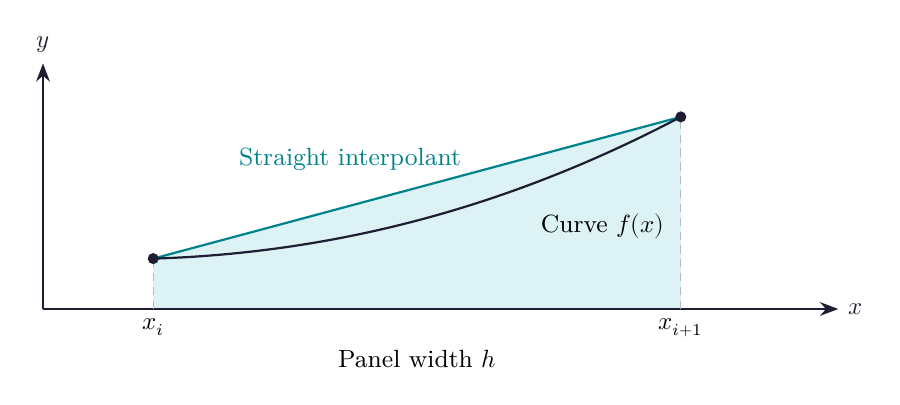
\begin{tikzpicture}[y=0.80cm,every node/.style={font=\small}]
  \fill[hdrteal] (1.4,0)--(8.1,0)--(8.1,3.05)--(1.4,0.8)--cycle;
  \draw[arrow] (0,0)--(10.1,0) node[right] {$x$};
  \draw[arrow] (0,0)--(0,3.9) node[above] {$y$};
  \draw[myteal,thick] (1.4,0.8)--(8.1,3.05);
  \draw[mydark,thick] (1.4,0.8) .. controls (4,0.9) and (6.2,1.8) .. (8.1,3.05);
  \draw[mgframe,densely dashed] (1.4,0)--(1.4,0.8) (8.1,0)--(8.1,3.05);
  \fill[mydark] (1.4,0.8) circle (2pt) (8.1,3.05) circle (2pt);
  \node[below] at (1.4,0) {$x_i$};
  \node[below] at (8.1,0) {$x_{i+1}$};
  \node[below] at (4.75,-0.5) {Panel width $h$};
  \node[above,text=myteal] at (3.9,2.04) {Straight interpolant};
  \node[right] at (6.2,1.32) {Curve $f(x)$};
\end{tikzpicture}\par
\end{tcolorbox}

\subsection{Simpson's one-third rule}
\begin{tcolorbox}[formulabox, title={Simpson weights and error}]
Use an even number $N$ of equal subintervals. On one two-subinterval panel, integrate the quadratic interpolant through $m-h,m,m+h$. Its three basis integrals are $h/3,4h/3,h/3$.
\[
S_N=\frac{h}{3}\left[y_0+y_N
    +4\!\!\!\sum_{\substack{1\le i<N\\ i\ \mathrm{odd}}}\!y_i
    +2\!\!\!\sum_{\substack{2\le i<N\\ i\ \mathrm{even}}}\!y_i\right].
\]
The panel error is $-h^5 f^{(4)}(\xi)/90$. The composite error is $I-S_N=-(b-a)h^4f^{(4)}(\xi)/180$ for continuous $f^{(4)}$. Here $h$ is one subinterval, so a single panel has width $2h$.
\end{tcolorbox}

\begin{enumerate}[leftmargin=*, itemsep=3pt, topsep=4pt]
  \item \textbf{Why the rule is exact through degree three.} It integrates the quadratic interpolant exactly. A cubic's remaining odd part about the midpoint contributes zero to both the integral and the symmetric weighted sum.
  \item \textbf{Where the error constant comes from.} Use the cubic Hermite interpolant that matches the three sampled values and the midpoint derivative. Its error factor, with $t=x-m$, is $(t+h)t^2(t-h)$. It has one sign across the panel.
  \item \textbf{Integrate the factor.} The Hermite remainder multiplies that factor by $f^{(4)}(\xi_x)/4!$. Integrating the factor gives $-4h^5/15$. Division by $4!$ yields $-h^5/90$, and summing $(b-a)/(2h)$ panels gives the composite constant.
\end{enumerate}
\begin{tcolorbox}[examplebox, title={Compare rules and their signed errors on the same data}]
Integrate $x^4$ from $0$ to $2$. Use $N=2$ and $h=1$, giving ordinates $0,1,16$.
\[
\begin{aligned}
I&=\frac{2^5}{5}=\frac{32}{5},\\
T_2&=\frac{0+16}{2}+1=9,\\
S_2&=\frac{0+4(1)+16}{3}=\frac{20}{3}.
\end{aligned}
\]
The signed errors are $I-T_2=-13/5$ and $I-S_2=-4/15$. With $f^{(4)}=24$, Simpson's formula agrees: $-2(24)/180=-4/15$.
\end{tcolorbox}

\newpage
\begin{center}
  {\large\bfseries\color{myred} Quick Revision --- Module 1}\\[3pt]
  {\small\color{mydark} Numerical Errors, Interpolation and Integration $|$ BS-M401}
\end{center}
\noindent{\color{myred}\rule{\linewidth}{1.2pt}}\par\vspace{4pt}

\begin{tcolorbox}[formulabox, title={Key Concepts at a Glance}]
\renewcommand{\arraystretch}{1.35}
\noindent\begin{tabularx}{\linewidth}{B{4.5cm}Y}
Signed error & $e=x-\hat x$. Relative error is $|e|/|x|$ when $x\ne0$. \\[3pt]
Error propagation & $\Delta g\approx\sum_i(\partial g/\partial x_i)\Delta x_i$. \\[3pt]
Newton offsets & $u=(x-x_0)/h$ for forward and $v=(x-x_n)/h$ for backward. \\[3pt]
Quadrature errors & Composite trapezoidal error is order $h^2$. Composite Simpson error is order $h^4$ under smoothness assumptions. \\[3pt]
\end{tabularx}\par
\end{tcolorbox}

\begin{tcolorbox}[defbox, title={One-Line Definitions}]
\begin{itemize}[leftmargin=*, itemsep=3pt, topsep=4pt]
  \item \textbf{Round-off.} Error introduced by finite digit storage or arithmetic.
  \item \textbf{Truncation.} Error introduced by replacing an exact procedure by a finite approximation.
  \item \textbf{Interpolation.} Estimate inside the sampled range.
  \item \textbf{Quadrature.} Approximate an integral using sampled function values.
\end{itemize}
\end{tcolorbox}

\begin{tcolorbox}[exambox, title={Frequently Asked / Viva Questions}]
\begin{enumerate}[topsep=0pt, label=\textbf{Q\arabic*.}, itemsep=5pt, leftmargin=*]
  \item \Q{Why can subtraction lose significant digits?}
    Errors in similar operands can dominate their small difference.
  \item \Q{What is the spacing with $f$ fixed binary fractional bits?}
    $2^{-f}$.
  \item \Q{What happens first in floating-point addition?}
    Align both significands to the same exponent.
  \item \Q{How does the first-order product error combine?}
    The signed relative changes add to first order.
  \item \Q{When is Newton forward preferred?}
    Nodes are equally spaced and the target is near the beginning.
  \item \Q{What changes in the Newton backward coefficients?}
    Use rising products in $v=(x-x_n)/h$ and differences at the last node.
  \item \Q{What is the advantage of Newton divided differences?}
    Unequal nodes are allowed, and another node adds a term to the existing polynomial.
  \item \Q{What is $L_i(x_j)$?}
    It is one if $i=j$ and zero otherwise.
  \item \Q{What subinterval count does composite Simpson require?}
    An even count of equal subintervals.
  \item \Q{What are the trapezoidal and Simpson degrees of exactness?}
    One and three, respectively.
  \item \Q{How does halving the step affect smooth composite error bounds?}
    The trapezoidal bound falls by a factor of four and the Simpson bound by sixteen under the same derivative bounds.
\end{enumerate}
\end{tcolorbox}

\begin{tcolorbox}[tikzbox, title={Summary Comparison}]
\par\vspace{5pt}
\begingroup
\setlength{\extrarowheight}{1pt}
\noindent\begin{tabularx}{\linewidth}{|B{3.45cm}|Y|Y|}
\hline
\textbf{Method} & \textbf{Where to apply} & \textbf{Check before using} \\ \hline
Newton forward or backward & Uniform nodes, near one end. & Choose the right end and maintain the sign of the offset. \\ \hline
Lagrange or divided differences & Any distinct nodes. & Keep the indices and node spacings in order. \\ \hline
Trapezoidal & Uniform composite grid for the stated formula. & Half-weight the endpoints. \\ \hline
Simpson one-third & Uniform grid with even subinterval count. & Use alternating weights 4 and 2 on the interior. \\ \hline
\end{tabularx}\par
\endgroup
\end{tcolorbox}


% -- Module 2 -----------------------------------------------------------------
\modulestart{2}{Linear Systems and Nonlinear Equations}

\section{Linear Systems and Nonlinear Equations}
\subsection{Linear systems, pivots and residuals}
\begin{tcolorbox}[defbox, title={Linear system}]
A square system $A\mathbf{x}=\mathbf{b}$ has a unique solution if $A$ is nonsingular. A \textbf{pivot} is the entry used to eliminate other entries in its column. After computing $\hat{\mathbf{x}}$, check the residual $\mathbf{r}=\mathbf{b}-A\hat{\mathbf{x}}$.
\end{tcolorbox}

\begin{itemize}[leftmargin=*, itemsep=3pt, topsep=4pt]
  \item \textbf{Direct methods.} Elimination, matrix inversion and LU solve a nonsingular system in finitely many arithmetic operations in exact arithmetic.
  \item \textbf{Iterative methods.} Gauss--Seidel improves an initial guess one sweep at a time. It needs a convergence condition and a stopping criterion.
  \item \textbf{Conditioning.} A small residual is a useful check. If $A$ is nearly singular, a small residual can still accompany a large solution error because $\mathbf{x}-\hat{\mathbf{x}}=A^{-1}\mathbf{r}$.
\end{itemize}

\subsection{Gauss elimination and back substitution}
\begin{enumerate}[leftmargin=*, itemsep=3pt, topsep=4pt]
  \item \textbf{Select a pivot.} At column $k$, partial pivoting chooses the largest absolute entry in that column from rows $k$ through $n$. Swap that row into position $k$, including the right-hand side.
  \item \textbf{Eliminate below.} For each $i>k$, set $m_{ik}=a_{ik}/a_{kk}$ and apply $R_i\leftarrow R_i-m_{ik}R_k$ to the augmented row.
  \item \textbf{Back-substitute.} For triangular system $U\mathbf{x}=\mathbf{c}$, solve
 \[
 x_i=\frac{c_i-\sum_{j=i+1}^n u_{ij}x_j}{u_{ii}},
 \qquad i=n,n-1,\ldots,1.
 \]
\end{enumerate}
A small pivot amplifies round-off. Partial pivoting keeps the elimination multipliers at magnitude at most one in that step. If the remaining pivot column is zero, the square system is not uniquely solvable. Use the augmented rows to distinguish inconsistency from free variables. Dense elimination costs $O(n^3)$ operations and back substitution costs $O(n^2)$.

\begin{tcolorbox}[examplebox, title={Gauss elimination with every row operation shown}]
Solve
\[
\left[\begin{array}{rrr|r}
2&1&1&7\\
4&3&3&19\\
8&7&9&49
\end{array}\right].
\]
For this exact-arithmetic hand example the available pivots are used as written.
\begin{enumerate}[leftmargin=*, itemsep=3pt, topsep=4pt]
  \item Apply $R_2\leftarrow R_2-2R_1$ and $R_3\leftarrow R_3-4R_1$. The lower rows become $(0,1,1\mid5)$ and $(0,3,5\mid21)$.
  \item Apply $R_3\leftarrow R_3-3R_2$. The last row is $(0,0,2\mid6)$.
  \item Back-substitute in the order $z,y,x$:
 \[
 \begin{aligned}
  z&=6/2=3,\\
  y&=5-z=2,\\
  x&=(7-y-z)/2=1.
 \end{aligned}
 \]
\end{enumerate}
Substitution into the original equations gives $(7,19,49)^{\mathsf T}$.
\end{tcolorbox}

\begin{tcolorbox}[masonbox, title={When pivoting is essential}]
For $\begin{pmatrix}0&1\\2&3\end{pmatrix}$, elimination cannot start with the top-left entry. Interchange the two rows first. The zero initial pivot does not make the matrix singular.
\end{tcolorbox}

\subsection{Matrix inversion by Gauss--Jordan elimination}
\begin{tcolorbox}[defbox, title={Gauss--Jordan inversion}]
Start with $[A\mid I]$. Perform the same elementary row operations on both halves until the left half becomes $I$. Divide each pivot row by its pivot and eliminate entries both above and below it. The right half is $A^{-1}$. This works because each row operation is left multiplication by an elementary matrix.
\end{tcolorbox}

\begin{tcolorbox}[examplebox, title={Invert a two-by-two matrix}]
Take $A=\begin{pmatrix}2&1\\1&1\end{pmatrix}$.
\begin{enumerate}[leftmargin=*, itemsep=3pt, topsep=4pt]
  \item Apply $R_2\leftarrow2R_2-R_1$ to $[A\mid I]$. The second row becomes $(0,1\mid-1,2)$.
  \item Subtract that row from row 1. The first row becomes $(2,0\mid2,-2)$.
  \item Divide row 1 by 2. The right block gives
 \[
 A^{-1}=\begin{pmatrix}1&-1\\-1&2\end{pmatrix}.
 \]
\end{enumerate}
Check $AA^{-1}=I$. The columns can also be found by solving $A\mathbf{x}_j=\mathbf{e}_j$. For a single right-hand side, elimination avoids computing an entire inverse.
\end{tcolorbox}

\subsection{LU factorisation and repeated right-hand sides}
\begin{tcolorbox}[defbox, title={Doolittle LU factorisation}]
Write $A=LU$ with a unit lower triangular $L$ and an upper triangular $U$. If row permutations are needed, use $PA=LU$. The elimination multipliers fill the entries below the diagonal of $L$.
\end{tcolorbox}

\begin{tcolorbox}[formulabox, title={Doolittle entry formulas}]
For column or row index $i=1,\ldots,n$, compute the row of $U$ first and then the column of $L$:
\[
\begin{aligned}
u_{ij}&=a_{ij}-\sum_{k<i} l_{ik}u_{kj}, && j\ge i,\\
l_{ji}&=\frac{a_{ji}-\sum_{k<i}l_{jk}u_{ki}}{u_{ii}}, && j>i,\\
l_{ii}&=1.
\end{aligned}
\]
Here $a_{ij}$ refers to the factorised matrix, with any required permutations applied. If pivoting is used, keep the permutation and the already stored multiplier columns consistent with the swaps.
\end{tcolorbox}

\begin{tcolorbox}[examplebox, title={Reuse the Gauss multipliers to solve the same system}]
The previous example had multipliers $2,4,3$ below the diagonal. Thus
\[
L=\begin{pmatrix}1&0&0\\2&1&0\\4&3&1\end{pmatrix},
\qquad
U=\begin{pmatrix}2&1&1\\0&1&1\\0&0&2\end{pmatrix}.
\]
\begin{enumerate}[leftmargin=*, itemsep=3pt, topsep=4pt]
  \item \textbf{Forward solve.} For $L\mathbf{y}=\mathbf{b}$, obtain $y_1=7$, $y_2=19-2(7)=5$, and $y_3=49-4(7)-3(5)=6$.
  \item \textbf{Backward solve.} Solving $U\mathbf{x}=(7,5,6)^{\mathsf T}$ gives $\mathbf{x}=(1,2,3)^{\mathsf T}$.
  \item \textbf{Reuse.} Each additional right-hand side needs two triangular solves. With pivoting, the first solve uses $P\mathbf{b}$.
\end{enumerate}
The one-time dense factorisation is $O(n^3)$. Each later solve costs $O(n^2)$.
\end{tcolorbox}

\subsection{Gauss--Seidel iteration}
\begin{tcolorbox}[formulabox, title={Use fresh values immediately}]
Given initial values $\mathbf{x}^{(0)}$, sweep through the equations in order. For a nonzero diagonal,
\[
x_i^{(k+1)}=\frac{1}{a_{ii}}
 \left(b_i-\sum_{j<i}a_{ij}x_j^{(k+1)}
           -\sum_{j>i}a_{ij}x_j^{(k)}\right).
\]
The lower-index variables use the current sweep. Jacobi would use the previous sweep for every variable.
\end{tcolorbox}

\begin{tcolorbox}[examplebox, title={Two sweeps of Gauss--Seidel}]
Solve
\[
4x+y+z=9,\quad 2x+5y+2z=18,\quad x+2y+4z=17
\]
from $(0,0,0)$. Rearrange to $x=(9-y-z)/4$, $y=(18-2x-2z)/5$, and $z=(17-x-2y)/4$.
\begin{enumerate}[leftmargin=*, itemsep=3pt, topsep=4pt]
  \item \textbf{Sweep 1.} $x^{(1)}=9/4=2.25$. Use it in $y^{(1)}=(18-4.5)/5=2.70$. Use both fresh values in $z^{(1)}=(17-2.25-5.40)/4=2.3375$.
  \item \textbf{Sweep 2.} Update $x^{(2)}=(9-2.70-2.3375)/4=0.990625$. Next $y^{(2)}=2.268750$ and $z^{(2)}=2.867969$ after rounding the displayed value.
  \item \textbf{Check convergence.} Every diagonal magnitude exceeds the sum of the other magnitudes in its row. Continue until both the update and residual are acceptably small. The exact solution is $(1,2,3)$.
\end{enumerate}
\end{tcolorbox}

Strict row diagonal dominance is sufficient for convergence. Symmetric positive definiteness is another sufficient condition. Check $\max_i|x_i^{(k+1)}-x_i^{(k)}|$ and a residual tolerance such as $\|\mathbf{r}\|_\infty/\max(1,\|\mathbf{b}\|_\infty)$. Set a maximum sweep count to avoid infinite iteration.

\section{Roots of Nonlinear Algebraic Equations}
\subsection{Brackets, residuals and stopping rules}
\begin{tcolorbox}[defbox, title={Root and sign-changing bracket}]
A root $r$ satisfies $f(r)=0$. For continuous $f$ on $[a,b]$, the condition $f(a)f(b)<0$ guarantees at least one interior root. A zero endpoint is already a root. A root of even multiplicity may fail to produce a sign change.
\end{tcolorbox}

For all three examples use $f(x)=x^3-x-2$. Its endpoint values are $f(1)=-2$ and $f(2)=4$. Since $f'(x)=3x^2-1>0$ on $[1,2]$, exactly one root lies there.

\subsection{Bisection}
\begin{enumerate}[leftmargin=*, itemsep=3pt, topsep=4pt]
  \item \textbf{Halve.} Compute the midpoint $m=a+(b-a)/2$ and evaluate $f(m)$.
  \item \textbf{Keep the bracket.} If $f(m)=0$ stop. If $f(a)f(m)<0$ keep $[a,m]$. Otherwise keep $[m,b]$.
  \item \textbf{Bound the error.} For the $k$th midpoint from the initial interval $[a_0,b_0]$, $|m_k-r|\le(b_0-a_0)/2^k$. For error at most $\varepsilon$, use at least $\max(1,\lceil\log_2((b_0-a_0)/\varepsilon)\rceil)$ midpoint evaluations.
\end{enumerate}
\begin{tcolorbox}[examplebox, title={Bisection on the cubic}]
\par\vspace{5pt}
\begingroup
\setlength{\extrarowheight}{1pt}
\noindent\begin{tabularx}{\linewidth}{|B{1.25cm}|Y|Y|Y|}
\hline
\textbf{Step} & \textbf{Midpoint} & \textbf{$f(m)$} & \textbf{Bracket kept} \\ \hline
1 & $1.5$ & $-0.125$ & $[1.5,2]$ \\ \hline
2 & $1.75$ & $1.609375$ & $[1.5,1.75]$ \\ \hline
3 & $1.625$ & $0.666015625$ & $[1.5,1.625]$ \\ \hline
\end{tabularx}\par
\endgroup
\end{tcolorbox}

\subsection{Regula-Falsi or false position}
\begin{tcolorbox}[formulabox, title={Chord intercept}]
Join $(a,f(a))$ and $(b,f(b))$ by a straight line. Setting the line's value to zero gives
\[
c=b-\frac{f(b)(b-a)}{f(b)-f(a)}
 =\frac{a f(b)-b f(a)}{f(b)-f(a)}.
\]
Update the bracket by the same sign test as bisection. Unlike a midpoint, the chord intercept is closer to an endpoint whose function value is smaller in magnitude.
\end{tcolorbox}

\begin{tcolorbox}[examplebox, title={False-position iterations on the cubic}]
From $[1,2]$,
\[
c_1=\frac{1(4)-2(-2)}{4-(-2)}=\frac{4}{3}.
\]
Since $f(4/3)=-26/27<0$, replace the lower endpoint. The next intercepts are $c_2\approx1.462687$ and $c_3\approx1.504019$. Their residuals are approximately $-0.333339$ and $-0.101818$, so $b=2$ stays fixed. False position may keep the same endpoint for many iterations. Its width does not necessarily halve, so the bisection error bound does not apply.
\end{tcolorbox}

\subsection{Newton--Raphson method}
\begin{tcolorbox}[formulabox, title={Tangent intercept}]
Linearise at $x_k$ and set the linear estimate to zero:
\[
0\approx f(x_k)+f'(x_k)(x_{k+1}-x_k)
 \quad\Longrightarrow\quad
x_{k+1}=x_k-\frac{f(x_k)}{f'(x_k)}.
\]
This needs $f'(x_k)\ne0$. It does not maintain a bracket unless an additional safeguard is used.
\end{tcolorbox}

\begin{tcolorbox}[examplebox, title={Newton iterates and a numerical stopping check}]
For the cubic, start with $x_0=1.5$. Then
\[
x_1=1.5-\frac{-0.125}{5.75}\approx1.521739130.
\]
Retaining working digits, $x_2\approx1.521379806$ and $x_3\approx1.521379707$. The residual at $x_2$ is about $5.89\times10^{-7}$. Report the root to the requested accuracy after checking the change in $x$ and the residual.
\end{tcolorbox}

\begin{tcolorbox}[masonbox, title={Convergence near the root}]
For a smooth function with a simple root $r$ and a sufficiently close start, Taylor expansion about $x_k$ gives
\[
x_{k+1}-r=\frac{f''(\xi)}{2f'(x_k)}(x_k-r)^2
\]
for some $\xi$ between $x_k$ and $r$. This explains quadratic local convergence. At a multiple root the usual iteration can converge only linearly. A poor start or a tiny derivative can take the next iterate far away.
\end{tcolorbox}

\begin{tcolorbox}[tikzbox, title={Bracket, chord and tangent choices}]
\centering
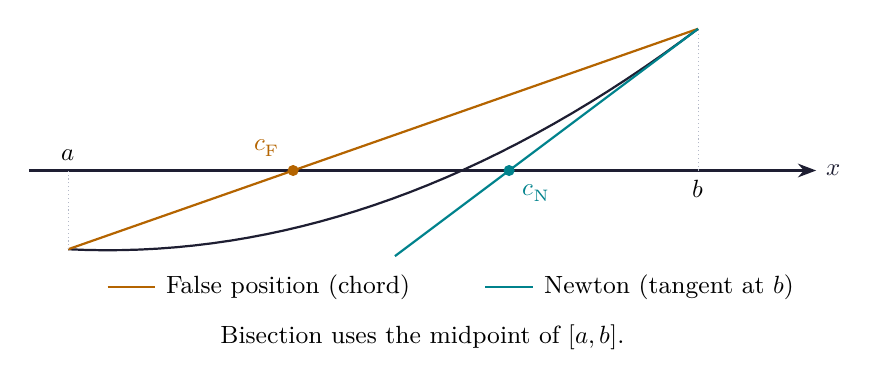
\begin{tikzpicture}[every node/.style={font=\small}]
  \draw[arrow] (-0.5,0)--(9.5,0) node[right] {$x$};
  \draw[mydark,thick,domain=0:8,samples=36] plot (\x,{0.05*(\x-5)*(\x+4)});
  \draw[myamber,thick] (0,-1)--(8,1.8);
  \draw[myteal,thick] (4.15,-1.0875)--(8,1.8);
  \draw[mgframe,densely dotted] (0,-1)--(0,0) (8,0)--(8,1.8);
  \fill[myamber] (2.857,0) circle (2pt);
  \fill[myteal] (5.6,0) circle (2pt);
  \node[above] at (0,0) {$a$};
  \node[below] at (8,0) {$b$};
  \node[above left=2pt,text=myamber] at (2.857,0) {$c_{\mathrm F}$};
  \node[below right=2pt,text=myteal] at (5.6,0) {$c_{\mathrm N}$};
  \draw[myamber,thick] (0.5,-1.48)--(1.1,-1.48);
  \node[right] at (1.12,-1.48) {False position (chord)};
  \draw[myteal,thick] (5.3,-1.48)--(5.9,-1.48);
  \node[right] at (5.92,-1.48) {Newton (tangent at $b$)};
  \node at (4.5,-2.12) {Bisection uses the midpoint of $[a,b]$.};
\end{tikzpicture}\par
\end{tcolorbox}

\newpage
\begin{center}
  {\large\bfseries\color{myred} Quick Revision --- Module 2}\\[3pt]
  {\small\color{mydark} Linear Systems and Nonlinear Equations $|$ BS-M401}
\end{center}
\noindent{\color{myred}\rule{\linewidth}{1.2pt}}\par\vspace{4pt}

\begin{tcolorbox}[formulabox, title={Key Concepts at a Glance}]
\renewcommand{\arraystretch}{1.35}
\noindent\begin{tabularx}{\linewidth}{B{4.5cm}Y}
Gauss multiplier & $m_{ik}=a_{ik}/a_{kk}$ and $R_i\leftarrow R_i-m_{ik}R_k$. \\[3pt]
LU solve & $PA=LU$ then $L\mathbf{y}=P\mathbf{b}$ and $U\mathbf{x}=\mathbf{y}$. \\[3pt]
Gauss--Seidel & Use the newly updated components in the same sweep. \\[3pt]
Bisection bound & The $k$th midpoint error is at most $(b_0-a_0)/2^k$. \\[3pt]
Newton update & $x_{k+1}=x_k-f(x_k)/f'(x_k)$. \\[3pt]
\end{tabularx}\par
\end{tcolorbox}

\begin{tcolorbox}[defbox, title={One-Line Definitions}]
\begin{itemize}[leftmargin=*, itemsep=3pt, topsep=4pt]
  \item \textbf{Pivot.} Entry used to remove other entries in a column.
  \item \textbf{Residual.} $\mathbf{b}-A\hat{\mathbf{x}}$ for a computed linear solution.
  \item \textbf{Bracket.} An interval containing a root, certified here by continuity and opposite endpoint signs.
  \item \textbf{False position.} Root estimate at the chord's intersection with the horizontal axis.
\end{itemize}
\end{tcolorbox}

\begin{tcolorbox}[exambox, title={Frequently Asked / Viva Questions}]
\begin{enumerate}[topsep=0pt, label=\textbf{Q\arabic*.}, itemsep=5pt, leftmargin=*]
  \item \Q{Why use partial pivoting?}
    It avoids zero pivots when a usable row exists and limits elimination multipliers.
  \item \Q{How do Gauss and Gauss--Jordan differ?}
    Gauss removes entries below pivots first. Gauss--Jordan also removes entries above the pivots and scales them to one.
  \item \Q{Why does LU help with many right-hand sides?}
    Keep the same factors and solve two triangular systems for each new vector.
  \item \Q{How is Gauss--Seidel different from Jacobi?}
    It uses newly computed values immediately.
  \item \Q{Name a sufficient Gauss--Seidel convergence condition.}
    Strict diagonal dominance by rows.
  \item \Q{What is checked before bisection?}
    Continuity, endpoint roots, and a sign change when neither endpoint is a root.
  \item \Q{What controls the bisection error?}
    The width of the interval before the midpoint is computed.
  \item \Q{Why can Regula-Falsi be slow?}
    One endpoint can remain fixed for many steps.
  \item \Q{What geometric line is used by Newton?}
    The tangent at the current estimate.
  \item \Q{What happens if Newton's derivative vanishes?}
    The update is undefined. Change the estimate or use a safeguarded method.
  \item \Q{What is a useful final check on a computed root?}
    Inspect the residual and a justified error or step tolerance.
\end{enumerate}
\end{tcolorbox}

\begin{tcolorbox}[tikzbox, title={Summary Comparison}]
\par\vspace{5pt}
\begingroup
\setlength{\extrarowheight}{1pt}
\noindent\begin{tabularx}{\linewidth}{|B{3.45cm}|Y|Y|}
\hline
\textbf{Method} & \textbf{What it needs} & \textbf{Main advantage} \\ \hline
Gauss or LU & Nonsingular system and usable pivots. & Direct solve with a clear substitution order. \\ \hline
Gauss--Seidel & Initial guess and convergence conditions. & Uses simple sweeps and little extra memory. \\ \hline
Bisection or false position & Continuous function with a sign-changing bracket. & Maintains a bracket under sign updates. \\ \hline
Newton--Raphson & Derivative and suitable initial estimate. & Quadratic local speed for a simple root. \\ \hline
\end{tabularx}\par
\endgroup
\end{tcolorbox}


% -- Module 3 -----------------------------------------------------------------
\modulestart{3}{Numerical Solutions of Ordinary Differential Equations}

\section{Numerical Solutions of Ordinary Differential Equations}
\subsection{Initial values, boundary values and error orders}
\begin{tcolorbox}[defbox, title={Initial-value problem}]
For $y'=f(x,y)$ and $y(x_0)=y_0$, the equation specifies a slope at each point. Use steps of size $h$ to approximate the solution at grid nodes $x_n=x_0+nh$. An initial-value problem gives all required starting conditions at one point.
\end{tcolorbox}

\begin{itemize}[leftmargin=*, itemsep=3pt, topsep=4pt]
  \item \textbf{Initial values.} Euler, Runge--Kutta and predictor--corrector methods advance from known starting data.
  \item \textbf{Boundary values.} Conditions are specified at different points. For example, $y(a)=\alpha$ and $y(b)=\beta$ for a second-order equation lead to a coupled system on a grid.
  \item \textbf{Local defect.} Compare one numerical step started with exact data against the exact next value.
  \item \textbf{Global error.} Compare the accumulated numerical value with the true solution at a fixed endpoint as the step is refined. For a convergent order-$p$ method, the global error is $O(h^p)$ under the appropriate smoothness and stability assumptions.
\end{itemize}

\subsection{Euler's explicit method}
\begin{tcolorbox}[formulabox, title={Advance along the starting slope}]
The Taylor expansion is $y(x_n+h)=y(x_n)+h y'(x_n)+O(h^2)$. Keeping the first two terms gives
\[
y_{n+1}=y_n+h f(x_n,y_n).
\]
Euler has local defect $O(h^2)$ and global error $O(h)$.
\end{tcolorbox}

\begin{tcolorbox}[tikzbox, title={One Euler step}]
\centering
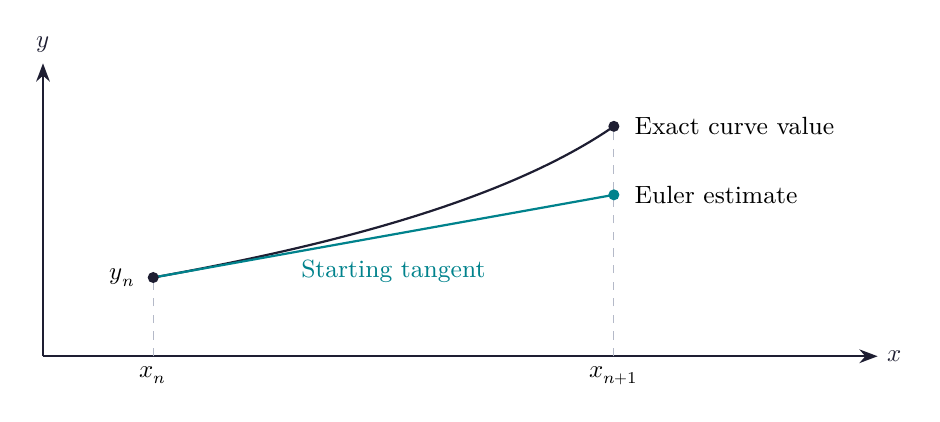
\begin{tikzpicture}[every node/.style={font=\small}]
\coordinate (a) at (1.4,1);
\coordinate (b) at (7.25,2.05);
\coordinate (c) at (7.25,2.92);
\draw[arrow] (0,0)--(10.6,0) node[right] {$x$};
\draw[arrow] (0,0)--(0,3.72) node[above] {$y$};
\draw[mgframe,dashed] (1.4,0)--(a) (7.25,0)--(c);
\draw[mydark,thick] (a) .. controls (3.4,1.36) and (5.8,1.92) .. (c);
\draw[myteal,thick] (a)--(b);
\fill[mydark] (a) circle (2pt) (c) circle (2pt);
\fill[myteal] (b) circle (2pt);
\node[left=3pt] at (a) {$y_n$};
\node[right=4pt] at (b) {Euler estimate};
\node[right=4pt] at (c) {Exact curve value};
\node[below] at (1.4,0) {$x_n$};
\node[below] at (7.25,0) {$x_{n+1}$};
\node[below,text=myteal] at (4.45,1.35) {Starting tangent};
\end{tikzpicture}\par
\end{tcolorbox}

\begin{tcolorbox}[examplebox, title={Compute two Euler steps}]
For $y'=x+y$, $y(0)=1$, use $h=0.1$.
\[
\begin{aligned}
y_1&=1+0.1(0+1)=1.10,\\
y_2&=1.10+0.1(0.1+1.10)=1.22.
\end{aligned}
\]
The exact solution is $2e^x-x-1$. At $x=0.2$ it is about $1.242806$, so the signed error (exact minus computed) is about $0.022806$.
\end{tcolorbox}

\begin{tcolorbox}[masonbox, title={Stability check}]
For $y'=\lambda y$, Euler multiplies the solution by $1+h\lambda$ in each step. For real $\lambda<0$, numerical decay requires $|1+h\lambda|<1$, or $0<h<2/|\lambda|$. An accurate order estimate applies when the step is sufficiently small.
\end{tcolorbox}

\subsection{Runge--Kutta methods}
Runge--Kutta evaluates several slopes within one step. In these formulas each $k_i$ is a slope, with the factor $h$ applied separately.

\begin{tcolorbox}[formulabox, title={Two second-order methods}]
\[
\begin{aligned}
\text{Heun:}\quad k_1&=f(x_n,y_n),\\
k_2&=f(x_n+h,y_n+hk_1),&
y_{n+1}&=y_n+\frac h2(k_1+k_2),\\[3pt]
\text{Midpoint:}\quad k_1&=f(x_n,y_n),\\
k_2&=f(x_n+h/2,y_n+hk_1/2),&
y_{n+1}&=y_n+hk_2.
\end{aligned}
\]
Both have local defect $O(h^3)$ and global error $O(h^2)$ for smooth problems.
\end{tcolorbox}

\begin{tcolorbox}[examplebox, title={One RK2 step using both forms}]
For the previous IVP, $k_1=1$ and $h=0.1$.
\begin{itemize}[leftmargin=*, itemsep=3pt, topsep=4pt]
  \item \textbf{Heun.} Predict the endpoint $(0.1,1.1)$. Its slope is $1.2$. The average gives $1+0.05(1+1.2)=1.11$.
  \item \textbf{Midpoint.} Predict $(0.05,1.05)$. Its slope is $1.10$, so the update gives $1+0.1(1.10)=1.11$.
\end{itemize}
The two different formulas happen to return the same first step on this IVP.
\end{tcolorbox}

\begin{tcolorbox}[formulabox, title={Classical fourth-order Runge--Kutta}]
\[
\begin{aligned}
k_1&=f(x_n,y_n),\\
k_2&=f(x_n+h/2,y_n+hk_1/2),\\
k_3&=f(x_n+h/2,y_n+hk_2/2),\\
k_4&=f(x_n+h,y_n+hk_3),\\
y_{n+1}&=y_n+\frac h6(k_1+2k_2+2k_3+k_4).
\end{aligned}
\]
The local defect is $O(h^5)$ and the global error is $O(h^4)$ for a smooth IVP under standard assumptions. The first midpoint slope supplies the second midpoint stage.
\end{tcolorbox}

\begin{tcolorbox}[examplebox, title={RK4 stage table on the same IVP}]
\par\vspace{5pt}
\begingroup
\setlength{\extrarowheight}{1pt}
\noindent\begin{tabularx}{\linewidth}{|B{1.7cm}|Y|Y|Y|}
\hline
\textbf{Stage} & \textbf{$x$ input} & \textbf{$y$ input} & \textbf{Slope $f=x+y$} \\ \hline
$k_1$ & $0$ & $1$ & $1$ \\ \hline
$k_2$ & $0.05$ & $1.05$ & $1.10$ \\ \hline
$k_3$ & $0.05$ & $1.055$ & $1.105$ \\ \hline
$k_4$ & $0.10$ & $1.1105$ & $1.2105$ \\ \hline
\end{tabularx}\par
\endgroup
\[
\begin{aligned}
y_1&=1+\frac{0.1}{6}(1+2.20+2.21+1.2105)\\
   &\approx1.110341667.
\end{aligned}
\]
The exact value at $0.1$ is about $1.110341836$. Keep working digits in the four slopes.
\end{tcolorbox}

\section{Predictor--Corrector Methods}
\subsection{The predict, evaluate, correct, evaluate sequence}
\begin{tcolorbox}[defbox, title={Predictor and corrector}]
A predictor uses known data to estimate the next value explicitly. A corrector uses a formula involving the slope at the new point. Use the predicted value to supply its first new-point slope.
\end{tcolorbox}

\begin{enumerate}[leftmargin=*, itemsep=3pt, topsep=4pt]
  \item \textbf{Predict.} Compute $y_{n+1}^{(p)}$ from stored values.
  \item \textbf{Evaluate.} Calculate $f_{n+1}^{(p)}=f(x_{n+1},y_{n+1}^{(p)})$.
  \item \textbf{Correct.} Compute $y_{n+1}^{(c)}$ using the predicted slope. If iteration is requested, repeat using the latest corrected slope until the change is suitably small.
  \item \textbf{Evaluate again.} Store $f(x_{n+1},y_{n+1}^{(c)})$ for future steps. The sequence is called PECE.
\end{enumerate}
A single-step pair uses Euler as predictor and $y_{n+1}^{(c)}=y_n+\tfrac h2(f_n+f_{n+1}^{(p)})$ as corrector. One correction gives Heun's method. Repeated corrections attempt to solve the implicit trapezoidal step. The multistep pairs below assume equal steps and require several accurate initial values. Use an accurate one-step method such as RK4 to generate them if needed.

\subsection{Adams--Bashforth and Adams--Moulton pair}
\begin{tcolorbox}[formulabox, title={Adams pair on a uniform grid}]
Let $f_j=f(x_j,y_j)$.
\[
\begin{aligned}
y_{n+1}^{(p)}&=y_n+\frac{h}{24}
 (55f_n-59f_{n-1}+37f_{n-2}-9f_{n-3}),\\
y_{n+1}^{(c)}&=y_n+\frac{h}{24}
 (9f_{n+1}^{(p)}+19f_n-5f_{n-1}+f_{n-2}).
\end{aligned}
\]
The predictor uses four old slopes. The fourth-order corrector uses the estimated new-point slope and the three latest old slopes.
\end{tcolorbox}

\subsection{Milne predictor and Simpson corrector}
\begin{tcolorbox}[formulabox, title={Milne--Simpson pair}]
\[
\begin{aligned}
y_{n+1}^{(p)}&=y_{n-3}+\frac{4h}{3}
 (2f_{n-2}-f_{n-1}+2f_n),\\
y_{n+1}^{(c)}&=y_{n-1}+\frac{h}{3}
 (f_{n-1}+4f_n+f_{n+1}^{(p)}).
\end{aligned}
\]
The corrector integrates the slope from $x_{n-1}$ to $x_{n+1}$ using Simpson weights. Start it from $y_{n-1}$.
\end{tcolorbox}

\begin{tcolorbox}[examplebox, title={Compare both pairs on one new node}]
For $y'=y$, $y(0)=1$ and $h=0.1$, use the exact starting values $y_j=e^{0.1j}$ for $j=0,1,2,3$. Then $f_j=y_j$. Use the formulas above to compute $y_4$.
\par\vspace{5pt}
\begingroup
\setlength{\extrarowheight}{1pt}
\noindent\begin{tabularx}{\linewidth}{|B{3.5cm}|Y|Y|}
\hline
\textbf{Pair} & \textbf{Prediction} & \textbf{After one correction} \\ \hline
Adams & $1.491820456$ & $1.491824885$ \\ \hline
Milne--Simpson & $1.491820892$ & $1.491824721$ \\ \hline
\end{tabularx}\par
\endgroup
For Milne--Simpson substitute $y_2=f_2=1.221402758$, $f_3=1.349858808$ and $f_4^{(p)}=1.491820892$ into $y_2+(0.1/3)(f_2+4f_3+f_4^{(p)})$. The exact value $e^{0.4}$ is about $1.491824698$. All table entries are rounded after computation.
\end{tcolorbox}

\section{Finite Difference Method for Boundary Values}
\subsection{Centred derivatives and grid equations}
Use $x_i=a+ih$ and write $Y_i$ for the computed value. Subtract Taylor expansions at $x_i\pm h$ to approximate the first derivative. Add them to approximate the second derivative.
\begin{tcolorbox}[formulabox, title={Three-point centred formulas}]
\[
\begin{aligned}
y'(x_i)&=\frac{y(x_{i+1})-y(x_{i-1})}{2h}+O(h^2),\\
y''(x_i)&=\frac{y(x_{i-1})-2y(x_i)+y(x_{i+1})}{h^2}+O(h^2).
\end{aligned}
\]
Odd powers cancel in the sum and even powers cancel in the difference. These are truncation errors of the derivative formulas for smooth solutions.
\end{tcolorbox}

\begin{enumerate}[leftmargin=*, itemsep=3pt, topsep=4pt]
  \item \textbf{Discretise each interior row.} For $y''+p(x)y'+q(x)y=r(x)$, multiply by $h^2$ after replacing the derivatives:
 \[
 (1-hp_i/2)Y_{i-1}+(h^2q_i-2)Y_i+
       (1+hp_i/2)Y_{i+1}=h^2r_i.
 \]
  \item \textbf{Insert the boundary data.} Substitute $Y_0=\alpha$ and $Y_N=\beta$. Move their contributions to the right-hand side of the first and last interior rows.
  \item \textbf{Solve and check.} Each row uses three adjacent grid values, giving a tridiagonal matrix. Check the residual of the discrete equations and both boundary values.
\end{enumerate}
\begin{tcolorbox}[examplebox, title={Solve a boundary-value problem on a five-node grid}]
Take $y''=-2$ on $[0,1]$, $y(0)=y(1)=0$, and $h=1/4$. The interior equations, multiplied by $-h^2$, are
\[
\left[\begin{array}{rrr|r}
 2&-1&0&1/8\\
 -1&2&-1&1/8\\
 0&-1&2&1/8
\end{array}\right].
\]
By symmetry $Y_1=Y_3=a$ and $Y_2=b$, so $2a-b=1/8$ and $2b-2a=1/8$. The second equation gives $b=a+1/16$. Substitute into the first to obtain $a=3/16$ and $b=1/4$. The exact solution is $y=x(1-x)$. The values match at the nodes because the centred second difference is exact for a quadratic.
\end{tcolorbox}

\newpage
\begin{center}
  {\large\bfseries\color{myred} Quick Revision --- Module 3}\\[3pt]
  {\small\color{mydark} Numerical Solutions of Ordinary Differential Equations $|$ BS-M401}
\end{center}
\noindent{\color{myred}\rule{\linewidth}{1.2pt}}\par\vspace{4pt}

\begin{tcolorbox}[formulabox, title={Key Concepts at a Glance}]
\renewcommand{\arraystretch}{1.35}
\noindent\begin{tabularx}{\linewidth}{B{4.5cm}Y}
Euler & $y_{n+1}=y_n+hf_n$. Global order one. \\[3pt]
RK2 & Two slopes per step. Heun averages endpoint slopes and midpoint uses a midpoint estimate. \\[3pt]
RK4 & Weights $1,2,2,1$ on the slopes, with multiplier $h/6$. \\[3pt]
Predictor--corrector & Predict, evaluate, correct, then evaluate again. \\[3pt]
Centred second difference & $(Y_{i-1}-2Y_i+Y_{i+1})/h^2$. \\[3pt]
\end{tabularx}\par
\end{tcolorbox}

\begin{tcolorbox}[defbox, title={One-Line Definitions}]
\begin{itemize}[leftmargin=*, itemsep=3pt, topsep=4pt]
  \item \textbf{IVP.} Known conditions at the starting point.
  \item \textbf{BVP.} Conditions specified at different points.
  \item \textbf{Local defect.} Error from one update started with exact data.
  \item \textbf{Stencil.} Grid locations used to approximate a derivative.
\end{itemize}
\end{tcolorbox}

\begin{tcolorbox}[exambox, title={Frequently Asked / Viva Questions}]
\begin{enumerate}[topsep=0pt, label=\textbf{Q\arabic*.}, itemsep=5pt, leftmargin=*]
  \item \Q{How is Euler derived?}
    Keep the constant and first-derivative terms in the Taylor expansion.
  \item \Q{What is Euler's global order?}
    First order for a sufficiently smooth, well-posed IVP.
  \item \Q{What distinguishes the two midpoint stages of classical RK4?}
    The first uses the starting slope and the second uses the first midpoint slope.
  \item \Q{How many slopes does classical RK4 evaluate per step?}
    Four.
  \item \Q{What is the one-step local defect of RK4?}
    $O(h^5)$ for a sufficiently smooth problem.
  \item \Q{Why do multistep methods need starting values?}
    Their formulas use several previously computed slopes.
  \item \Q{How is the first slope used in the corrector found?}
    Evaluate the ODE at the predicted new-point value.
  \item \Q{Where does Milne's Simpson corrector start?}
    At $y_{n-1}$. Its integration panel spans $x_{n-1}$ to $x_{n+1}$.
  \item \Q{Why does the three-point stencil yield a tridiagonal system?}
    Each row relates the current node to its two neighbours.
  \item \Q{How are prescribed endpoints handled?}
    Substitute them into the outer interior rows and move the known terms to the right-hand side.
  \item \Q{Does a second-order stencil ensure a good answer on any grid?}
    Solution accuracy also depends on the step size, smoothness and stability of the discretisation.
\end{enumerate}
\end{tcolorbox}

\begin{tcolorbox}[tikzbox, title={Summary Comparison}]
\par\vspace{5pt}
\begingroup
\setlength{\extrarowheight}{1pt}
\noindent\begin{tabularx}{\linewidth}{|B{3.45cm}|Y|Y|}
\hline
\textbf{Method} & \textbf{Typical use} & \textbf{Main check} \\ \hline
Euler & Quick first-order IVP estimate. & Check accuracy and stability at the selected step. \\ \hline
Runge--Kutta & Accurate one-step IVP computation. & Keep stage locations and the slope convention consistent. \\ \hline
Predictor--corrector & Continue a uniformly spaced IVP solution. & Use accurate starting values and correct slope indices. \\ \hline
Finite difference & Assemble a BVP system. & Insert both endpoint conditions. \\ \hline
\end{tabularx}\par
\endgroup
\end{tcolorbox}


\end{document}
